\documentclass[12pt]{article}
\usepackage[margin=1in]{geometry}
\usepackage[all]{xy}


\usepackage{amsmath,amsthm,amssymb,color,latexsym}
\usepackage{geometry}        
\geometry{letterpaper}    
\usepackage{graphicx}

\usepackage{listings}
\usepackage{xcolor}

\usepackage[export]{adjustbox}

\definecolor{codegreen}{rgb}{0,0.6,0}
\definecolor{codegray}{rgb}{0.5,0.5,0.5}
\definecolor{codepurple}{rgb}{0.58,0,0.82}
\definecolor{backcolour}{rgb}{0.95,0.95,0.92}

\lstdefinestyle{mystyle}{
  backgroundcolor=\color{backcolour},   commentstyle=\color{codegreen},
  keywordstyle=\color{magenta},
  numberstyle=\tiny\color{codegray},
  stringstyle=\color{codepurple},
  basicstyle=\ttfamily\footnotesize,
  breakatwhitespace=false,         
  breaklines=true,                 
  captionpos=b,                    
  keepspaces=true,                 
  numbers=left,                    
  numbersep=5pt,                  
  showspaces=false,                
  showstringspaces=false,
  showtabs=false,                  
  tabsize=2
}

\lstset{style=mystyle}

\usepackage{graphicx}
\graphicspath{ {./images/} }


\newtheorem{problem}{Problem}

\newenvironment{solution}[1][\it{Solution}]{\textbf{#1. } }{$\square$}


\begin{document}
\noindent MATH 7233: Graph Theory, Fall 2021\hfill Homework Assignment \#1\\
Anjali, Nathan, Sai Nikhil\hfill 10/06/2021

\hrulefill

\begin{problem}
In a small Graph Theory class with 9 students everyone was asked how many of their friends are also taking the class.  Friendship is mutual.  Which of the following sets of answers could possibly be the actual outcome?  All three?  Perhaps none?*(c)  7,7,7,6,3,3,3,2,2?
\end{problem}

\begin{proof}
Suppose such a graph exists.

Let $X = $ No. of edges from A to B, where the vertices are sorted into two groups A and B as follows:

\begin{center}
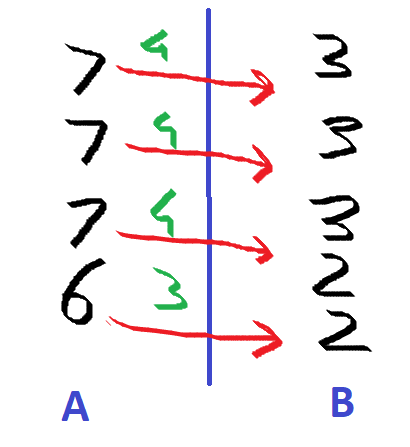
\includegraphics[scale=0.75]{WS_1}    
\end{center}

We see that the vertices of degree 7 connect to at most 3 people from group A. Now, each has at least 4 edges coming out of it which have to be connected to group B. If does not connect with people from group A, then it has to have more than 4 edges coming out of it. Similarly, the vertex of degree 6 has at least 3 edges coming out of it.
So now,\\
 $X \geq 4+4+4+3$
\\
i.e $X \geq 15$\\

However, B can accommodate only 3+3+3+2+2=13 edges. So, X should be $\leq 13$.\\
i.e $13 \geq X \geq 15$\\
This is not possible.\\
Hence no such graph can exist.

\end{proof}


\begin{problem}
Middle-Earth  -  after  the  global  warming  induced  by  the  One  Ring  being  thrown  into  the abyss  of  Mt  Doom  -  consisted  of  1000  little  islands.   Two  airlines  provided  transportation between the islands:  ElvenAir and AirDwarf.  Between any two islands there was a single,daily non-stop flight in both directions, operated by one of the two airlines.  But which islands were connected by which airlines was a mess.Gandalf wanted join the loyalty program of one of the airlines, and then stick to that one.At the same time he wanted to be able to travel freely between all the islands.  Fortunately he didn’t mind multiple layovers.  Can we be certain that he was able to pull it off?
\end{problem}

\begin{solution}
Induction Hypothesis: For K islands we can find an airline that connects all the islands.\\
Induction step: For K+1 island we can find an airline that connects all the islands.\\
Start with a graph with K+1 nodes.

\begin{center}
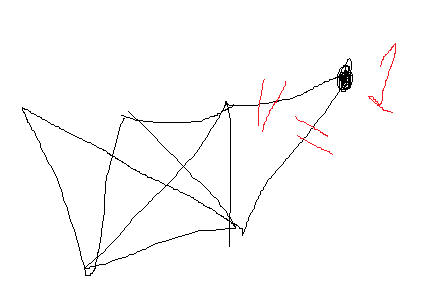
\includegraphics[scale=0.75]{WS_1_3}    
\end{center}

Remove node 1 and all its edges. This new graph has V’ vertices and E’ edges.\\
i.e G’=(V’E’)\\
G’ has K nodes. We can find an airline that connects all nodes. This is induction hypothesis.\\
Now bring back node 1:\\
Case 1: Node 1 is connected to G’ by only airline 1 and 2. So pick either airline 1 or 2.\\
Case 2: Node 1 is connected by airline 1 or by airline 2, so we will pick airline 1 or airline 2.\\

\end{solution}


\begin{problem}
Show that any graph in which every degree is at least 2 contains a cycle.
\end{problem}

\begin{proof}
Let $G$ be a graph in which every degree is at least 2. Suppose $P$ is a path of maximal length in $G$, ending with some node $v$. Since $v$ is the last node in $P$, there is exactly one edge incident to $v$ in $P$. But $v$ has degree at least 2, meaning there is some other edge $e$ incident to $v$ which is not in $P$. If $e$ is an edge between $v$ and some node $u$ which is not in $P$, then $P$ could be extended to also include $e$, contradicting the assumption that $P$ is maximal. Therefore, the node $u$ must already be in $P$. So the portion of $P$ from $u$ to $v$ along with $e$ is a cycle in $G$. Thus, any graph in which every degree is at least 2 must contain a cycle.
\end{proof}


\begin{problem}
Show that a CCF graph on $n$ vertices has exactly $n-1$ edges! (Hint: use induction on $n$.)
\end{problem}

\begin{proof}
First, let $G$ be a CCF graph with 1 vertex. Then clearly, $G$ must have 0 edges, as any simple graph with one vertex cannot have any edges. So the statement holds for the case $n=1$.

Now assume the statement holds for CCF graphs with $k-1$ vertices and consider a CCF graph $G$ on $k$ vertices. We claim that $G$ must have a vertex of degree exactly 1. Indeed, by 2.2, for $G$ to be cycle free, it must have some vertex $v$ with degree less than 2. Since $G$ is connected, the degree of $v$ cannot be 0, so it must be exactly 1.

Consider the subgraph $H$ of $G$ obtained by removing $v$. Notice that $H$ has $k-1$ vertices. We claim that $H$ is a CCF graph. There are no cycles in $G$ and removing a vertex cannot create a cycle since no new edges are created, so $H$ is cycle free. Furthermore, it is connected: given any two vertices $v_1$ and $v_2$ other than $v$ in $G$, there is some path between them in $G$ since $G$ is assumed to be connected. This path cannot contain $v$, since any path that includes a degree 1 vertex must start or end there. Therefore, this path still exists in $H$, meaning there is a path in $H$ between any two vertices of $H$. So $H$ is connected and thus a CCF graph.

We can now apply the inductive hypothesis. Since $H$ is a CCF graph on $k-1$ vertices, we know that it has $k-2$ edges. But then $G$ must have $k-1$ edges, since its set of edges consists exactly of the edges in $H$ and the additional single edge incident to $v$. We conclude that the statement must also hold for CCF graphs on $k$ vertices, so by induction, a CCF graph on $n$ vertices has exactly $n-1$ edges for any positive integer $n$.
\end{proof}


\begin{problem}
Show that any connected graph contains a \textit{connecting CCF subgraph}: a subgraph that is CCF and has the same number of vertices as the original graph. (Hint: are there any edges you can throw away without disconnecting the graph?)
\end{problem}

\begin{proof}
First, we claim that given a connected graph $G$, removing an edge from a cycle in $G$ results in a connected subgraph. Given a cycle $C$ in $G$, consider an edge $e$ between two vertices $v_1$ and $v_2$ in $G$. There must also be a path between $v_1$ and $v_2$ consisting of all the edges in the cycle other than $e$. So $C - e$ is a path between $v_1$ and $v_2$ which will contain every vertex in the cycle, meaning there is a path in $C - e$ between any two vertices in $C$. So now consider any two vertices in $G$. Because $G$ is connected, there is some path between them in $G$. If this path does not contain $e$, then it still exists in the subgraph $G - e$. Otherwise, the path must intersect the cycle $C$, beginning at some vertex $u_1$ in $C$ and ending at some vertex $u_2$ in $C$. But there is a path in $C - e$ between $u_1$ and $u_2$ so by replacing the part of the original path which intersects $C$ with this new path contained in $C-e$, one obtains a new path between the two vertices which is contained in $G-e$. Therefore, any two vertices in $G-e$ have a path between them, so $G-e$ is still connected. Furthermore, $G-e$ has the same vertex set as $G$.

Now consider the following algorithm: if $G$ has a cycle $C$, remove an edge from it to get another connected graph. Continue removing edges in this way until $G$ has no cycles remaining. We note that because a graph has a finite number of edges, it must have a finite number of cycles as well, so this process must terminate, as the number of cycles is strictly decreasing at each step. The subgraph of $G$ obtained by this algorithm has no cycles and must be connected, as we have seen that removing edges in this way from a connected graph always results in a connected graph. So this subgraph is CCF and must have the same number of vertices as $G$, meaning it is the desired subgraph.
\end{proof}

\begin{problem}
Show that any group of people can be arranged in two rooms such that each person has at most as many friends in their own room group than in the other room.
\end{problem}
\begin{proof}

\textbf{Proof by Algorithm:}

Let us have two divisions of students, such that initially all the students are in room 1 and the room 2 is empty as follows:

\begin{center}
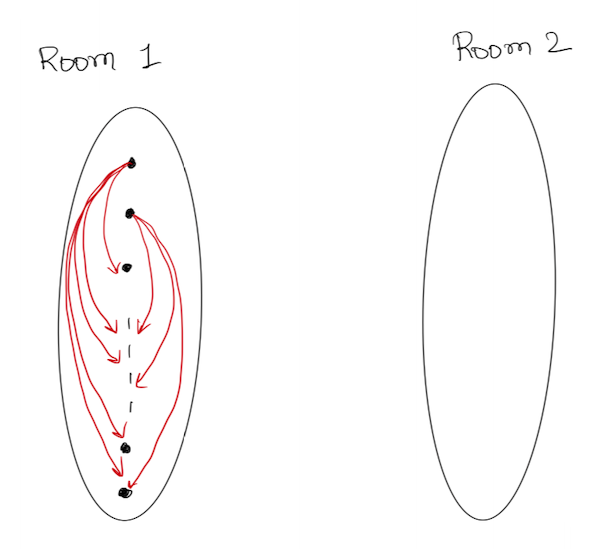
\includegraphics[width=16cm, keepaspectratio]{1}
\end{center}

Let us consider $n$ nodes in the graph, initially all in room 1 and none in room 2 with certain violations. We can move person $i$ to room 2 in order to migitate number of violations. At this point the split looks like the following:

\begin{center}
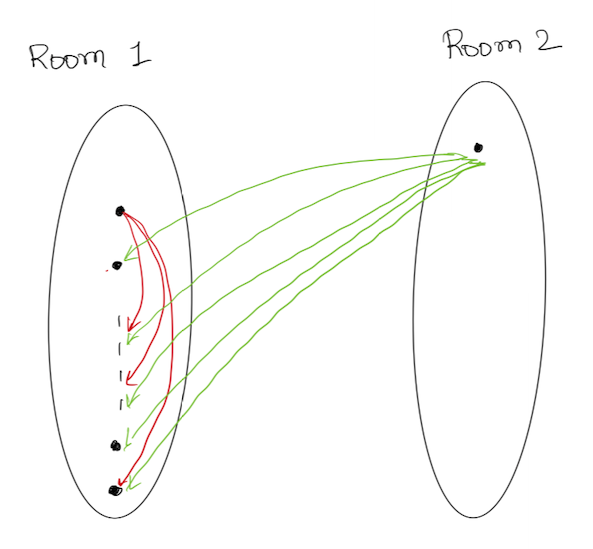
\includegraphics[width=16cm, keepaspectratio]{2}
\end{center}

Similarly, we can move person $j$ to room 2 if he's violating the principle of more crossing edges than in group edges. This process can be continued till we have no violation.

If we observe closely, we are increasing the number of crossing edges in every iteration of our algorithm, which itself has a limit that it cannot exceed the total number of edges in the graph. Hence, this process should terminate. And we have a condition that this will terminate only when there are no violations. This means we also have a solution for the problem.

\end{proof}


\begin{problem}
Let $G$ be a graph on 10 vertices that has no triangles. Show that $G^{c}$ must have a $K_{4}$ sub-graph.
\end{problem}

\begin{proof}
Consider an arbitrary vertex $v$ in a graph $G$ with $10$ nodes. Let us consider the following cases:

\textbf{Case I:}

$deg(v) \ge 4$

\begin{center}
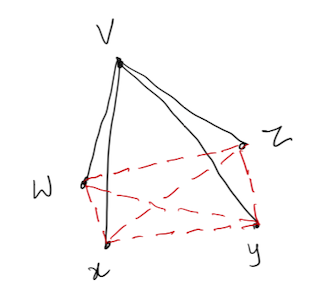
\includegraphics[width=16cm, keepaspectratio]{3}
\end{center}

Let, $v$ is connected to atleast $4$ other nodes $wxyz$. Because, $G$ has no triangles, no two nodes in $wxyz$ are connected. Hence, we have a $K_4$ in $G^{c}$, as highlighted in the above figure.
\\

\textbf{Case II:}

$deg(v) \le 4$

\begin{center}
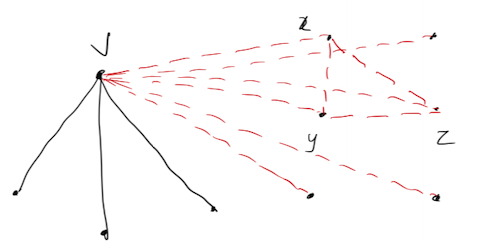
\includegraphics[width=16cm, keepaspectratio]{4}
\end{center}

Let, $v$ is connected to at max $3$ other nodes. This means there are at least $6$ other nodes where $v$ is connected to in $G^{c}$. From worksheet 1, we know in a graph $X$ of 6 nodes, either $X$ or $X^{c}$ has a triangle. In this case, let $X$ is a sub-graph formed by the above $6$ nodes. It has no triangle according to hypothesis. Hence, there must be a triangle in $X^{c}$ or rather $G^{c}$. Now, select those three vertices, say $xyz$. Along with $v$, there is a $K_4$, $vxyz$ as shown in figure above.



\end{proof}

\end{document}
